\documentclass[11pt]{article}

\usepackage[T2A]{fontenc}
\usepackage[utf8]{inputenc}
\usepackage[russian]{babel}

\usepackage{graphicx}
\usepackage{amsmath}
\usepackage{indentfirst}
\usepackage[nottoc]{tocbibind}
\usepackage{listings}
\usepackage{nameref}
\usepackage[usenames,dvipsnames]{xcolor}
\usepackage[center]{caption}

\lstset{
	backgroundcolor=\color{blue!4},
	commentstyle=\color{green!80},
    keywordstyle=\color{blue},
    stringstyle=\color{red},
	tabsize=4,
	basicstyle=\ttfamily
}

\setcounter{secnumdepth}{0}

\setlength{\parindent}{0em}
\setlength{\parskip}{1em}

\begin{document}	
	\begin{titlepage}
	\begin{figure}[t]
		\centering{
\includegraphics[width=0.3\textwidth]{images/uni-logo.png}}
	\end{figure}

	\begin{center}
		\textsc{\Large{Санкт-Петербургский государственный университет\\}}
		\textsc{\Large{Факультет прикладной математики --- процессов управления\\}}
		\textnormal{\Large{Программирование и информационные технологии\\}}
		\vspace{24mm}
		
		\Huge{Теория графов и её приложения}\\
		\LARGE{Отчёт по проектному заданию}
	\end{center}
	\vspace{19mm}
		
	\begin{minipage}[t]{0.38\textwidth}
		\textnormal{\large{\textbf{Преподаватели}\\}}
		\large{Воронкова Е. Б.}\\
		\large{Вольф Д. А.}
	\end{minipage}\hfill\begin{minipage}[t]{0.38\textwidth}\raggedleft
		\textnormal{\large{\textbf{Выполнили\\}}}
		\large{Козырев C. А.}\\
		\large{Куклин Д. В.}
	\end{minipage}
	\vspace{19mm}
		
	\centering{\large{Санкт-Петербург \\ 2020}}
	\pagebreak
    \end{titlepage}
    
    \tableofcontents
    \pagebreak
    
    \section{Постановка задачи и методы решения}
    
    В качестве семестрового проекта по теории графов требовалось, используя картографические данные проекта \textit{OpenStreetmap}, построить граф дорог Российского города-миллионера и выполнить задания по оценке удобства размещения зданий и планированию их размещения, используя построенный граф.
    
    Для реализации проекта мы выбрали язык C++, так как
    \begin{itemize}
    \item подавляющее большинство проектов для работы с картами написаны либо на C, либо на C++; либо используют линковку с Python, но также предоставляют C++ интерфейс,
    \item среди языков, которые используются в картографических проектах, C++ является наиболее быстрым,
    \item Python простой.
    \end{itemize}
    
    Также выбрали Нижний Новгород в качестве города-миллионера.
    
    Следуя условию задачи, мы использовали данные \textit{OpenStreetMap} (далее \textit{OSM}).
    
    \subsection{Построение графа дорог}
    
	Спецификация \textit{OSM} \cite{osm-main} определяет следующие структуры данных для хранения объектов географических карт: \textit{Node}, \textit{Way} и \textit{Relation} \cite{osm-wiki}.
	
	Структура \textit{Node} (узел) \cite{osm-node} обязана иметь уникальный идентификатор (\texttt{Integer}, занимающий 64 бита), а также широту и долготу (рекомендуется использовать \texttt{Float} шириной не менее 64 бит).
	Опционально каждый объект типа \textit{Node} содержит множество меток (\textit{tag}), которые позволяют получить дополнительную информацию об объекте карты (например, метка \textit{highway=crossing} даёт понять, что данный обозначает пешеходный переход).

	Структура \textit{Way} (путь) \cite{osm-way} есть упорядоченный список узлов, которая либо имеет по крайней мере одну метку, либо принадлежит \textit{Relation}.
    	Пути могут быть открытыми, либо закрытыми.
    	У открытых путей не совпадают первый и последний узлы.
    	Многие дороги определяются в \textit{OSM} как открытые пути.
    	
    	Закрытые пути как правило определяют объект \textit{Area} (к нему относятся дома, окольные пути, стены и т. п.).
    	
    	Структуру \textit{Relation} (отношение) мы исключили из рассмотрения, так как используемая нами библиотека не имеет широких возможностей для работы с ней.
    	Также, объекты этого типа по большей части не предоставляют требуемую нами информацию.
    
	Для работы с данными \textit{OSM} мы использовали библиотеку \textit{Libosmium} \cite{libosm}, которая предоставляет удобный API на языке C++ для работы с объектами \textit{OSM}.
	
	Первым шагом мы загрузили Protobuf файл карты Нижнего Новгорода с сайта-планировщика велосипедных путей \textit{BBBike} \cite{bbbike} (см. Рис. \ref{fig:bbbike}).

	\begin{figure}[ht]
	\centering	
	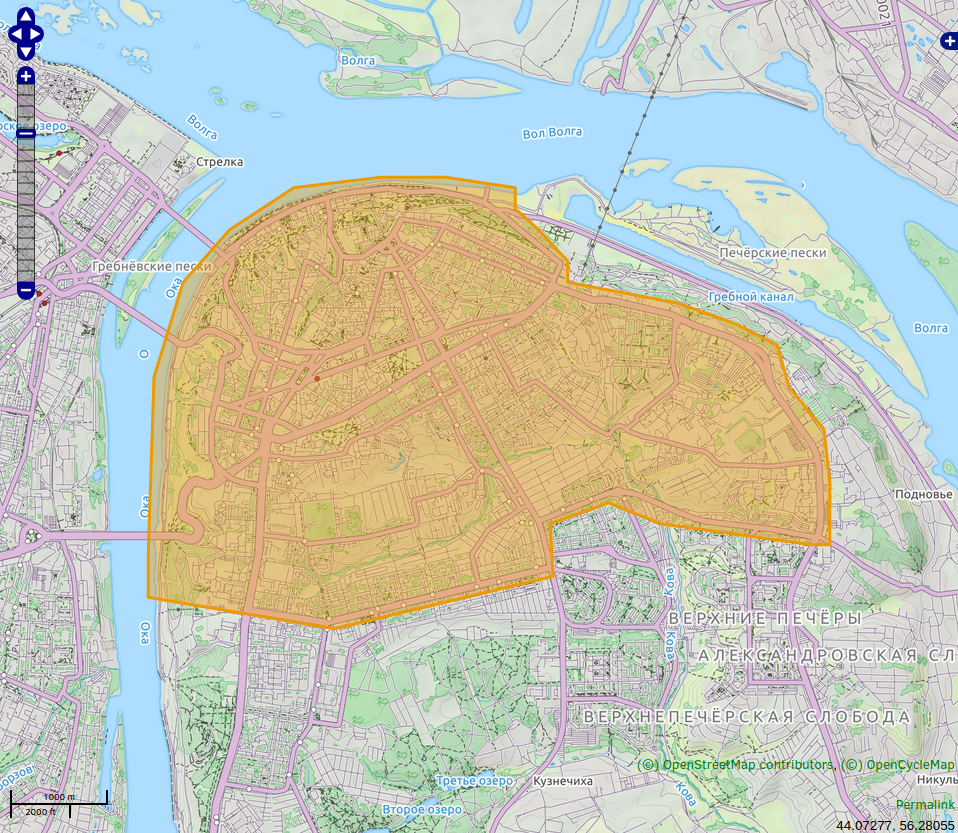
\includegraphics[width=0.8\textwidth]{images/bbbike.png}
	\caption{Используемая карта центра Нижнего Новгорода}
	\label{fig:bbbike}
	\end{figure}
	
	Далее требовалось создать карту узлов, используя \cite{libosm}.
	Задача осложнялась тем, что пути могли иметь пересечения в некоторых узлах, значит, необходимо было разделить пути по узлам, лежащим на пересечениях.
	Также, многие рёбра могли быть использованы без пользы, например в тупиках, но вносить весомый вклад в производительность.
	
	Мы использовали способ, предложенный на форуме \cite{forum}, что позволило сократить число узлов почти в два раза.
	Для простоты здесь и далее из кода убраны обозначения, не связанные с его логикой.
	
	\lstinputlisting[language=C++]{snippets/mark.cpp}
	
	Для каждого пути на карте мы помечали каждый узел пути, если он встречался более одного раза (таким образом, он лежит на пересечении).
	При следующей итерации по каждому пути, мы разделяли путь по узлу, имеющему отметку.
	Если узел не помечен, то в граф добавляем ребро между предыдущим и текущим узлами.
	
	Так как у каждого узла известна широта и долгота, то расстояние между двумя узлами можно вычислить, используя формулу гаверсинуса \cite{haversine}:
\begin{gather*}
	\eta(\Theta) = \eta(\varphi_2 - \varphi_1) + \cos(\varphi_1) \cos(\varphi_2) \eta(\lambda_2 - \lambda_1), \\
	d = 2r \arcsin(\sqrt{\eta(\Theta)}),
\end{gather*}
	где $ \Theta $~--- центральный угол, $ \varphi_{1,2} $~--- широты в радианах, $ \lambda_{1,2} $~--- высоты в радианах и $ \eta(\theta) = \sin^2 \left(\frac{\theta}{2}\right) $ для произвольного угла $ \theta $.
	
	\lstinputlisting[language=C++]{snippets/fill.cpp}
 	
	Структура \texttt{Node} содержит, как и в спецификации, поля уникального идентификатора в \textit{OSM}, широту и высоту.
 	
	\lstinputlisting[language=C++]{snippets/node.cpp}
 	
 	Граф представлен списком смежности.
 	
 	\lstinputlisting[language=C++]{snippets/graph.cpp}
 	
 	Так как и жилые дома, и объекты инфраструктуры определяются в \textit{OSM} как пути, то их сложно связать в одной структуре с графом дорог.
 	Для примера, мы могли помещать каждый узел здания в граф и помечать его особым образом, чтобы выделять среди узлов-частей дорог.
 	В таком случае усложнилась бы реализация большинства алгоритмов и вспомогательных структур.
 	
 	Мы решили выбрать иной подход к решению задачи.
	Для каждого здания на карте
	\begin{enumerate}
	\item вычисляем барицентр здания,
	\item находим ближайший к зданию узел дороги,
	\item в структуре \textit{Building} связываем со зданием найденный узел.
	\end{enumerate}
	
	\lstinputlisting[language=C++]{snippets/building.cpp}
	
	Финальная структура, содержащая всю необходимую информацию о карте города, имеет следующий вид:
	
	\lstinputlisting[language=C++]{snippets/map.cpp}
	
	Очевидно, что время составления карты оказывается довольно велико.
	Во-первых, библиотека \textit{Libosmium} каждый раз производит чтение файла с картой и последующее заполнение собственных объектов данных.
	Вопрос итоговой сложности всех библиотечных операций является открытым, но любой желающий может получить на него ответ, изучив исходный код библиотеки \cite{libosm-code}.
	
	Во-вторых, сложность составления карты равна $ O(n \cdot (m + n)) $, где $ m $~--- число узлов-домов, а $ n $~--- число узлов-дорог.
	Таким образом, даже при 16 тысячах узлов (примерное число узлов на карте центра Нижнего Новгорода), карта заполняется несколько минут, что неприемлемо для real-time приложения.
	
	Мы решили эту проблему, применив кэширование к полученной структуре данных \texttt{Map}.
	Для простоты реализации используем популярную библиотеку \textit{Boost}.
	
	\lstinputlisting[language=C++]{snippets/serialize.cpp}
	\lstinputlisting[language=C++]{snippets/deserialize.cpp}
	
	Подход оправдывает себя, так как большая часть карты остается статичной и при добавлении в базу данных новых узлов каждый раз заново обходить все пути не требуется.
	В итоге, скорость загрузки карты сократилась с нескольких минут до долей секунды (более точные измерения см. в \nameref{section:results}), и граф дорог Нижнего Новгорода построен.
	
    \subsection{Оценка удобства размещения объектов инфраструктуры}
    
    Требовалось выбрать $ M $ произвольных объектов инфраструктуры и $ N $ жилых зданий оценить удобство их размещения, используя расстояние как метрику.
    При обходе всех путей (\textit{Way} в \textit{OSM}), мы выбирали пути с соответствующими метками.
    
    \lstinputlisting[language=C++]{snippets/categories.cpp}
    
    Как было указано выше, для каждого здания мы запоминаем ближайший узел.
    
    \lstinputlisting[language=C++]{snippets/closest.cpp}
    
    Для определения кратчайших путей от объекта карты до другого естественным кажется применение алгоритма Дейкстры.
    Нами был реализован алгоритм с временной сложностью $ O(n \log n) $ (подробнее см. \nameref{section:results}).
    
    \lstinputlisting[language=C++]{snippets/dijkstra.cpp}
    
    Используя результаты работы алгоритма несложно как и определить ближайшие объекты, так и построить дерево кратчайших путей.
    
    \subsection{Планирование новых объектов}
    
    \section{Результаты}\label{section:results}
	
	\pagebreak

	\bibliographystyle{acm}
	\bibliography{report}
	
\end{document}
